\label{capitolo7}
\section{Sistemi termici}
Per qunto riguarda i sistemi temici ci occuperemo di alcuni materiali che dobbiamo specificare:
\begin{itemize}
\item vettore termico:un fluido incomprimibile con un calore specifico costante nell'intervallo di temperature interessate.
\item aria contenuta negli edifici: considerata alla stessa pressione di quella atmosferica
\item materiali solidi: entrano in gioco nel contenimento dei liquidi o dei gas, per essi basterà una semplice descrizione
\end{itemize}
\subsection{Componenti principali}
Analiziamo ora i componenti principali che entrano in gioco nei sistemi termici.
\subsubsection{Tubi}
\begin{figure}[tbh]
\centering
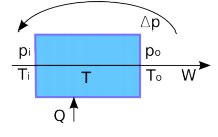
\includegraphics{img/tubo2.png}
\caption{Schema del tubo}
\label{fig:tubo2}
\end{figure}
Le equazioni idrauliche sono:
$$
\Delta p= \frac{K_T}{\rho}w^2-\rho g \Delta z
$$
Equazione di bilancio delle energie:
$$
\rho V c \dot{T_o}=cw(T_i-T_o)+Q
$$
\subsubsection{Pompe}
\begin{figure}[tbh]
\centering
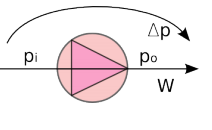
\includegraphics{img/pompa2.png}
\caption{Schema di una pompa}
\label{fig:pompa2}
\end{figure}
Esistono diversi tipi di pompe centrifughe o volumetriche, esse variano la loro portata in base alla loro velocità comandata dal valore $n$. I flussi di massa e di volume sono proporzionali alla densità $\rho$ e vengono indicati rispettivamente da $w$ e $q$.\\
Per quanto riguarda le pompe di tipo centrifugo:
$$
\Delta p= H0(n)-H1(n)w^2
$$
Mentre per quanto riguarda l'aspetto termico abbiamo che 
$$T_i=T_o$$
\subsubsection{Valvole}
\begin{figure}[tbh]
\centering
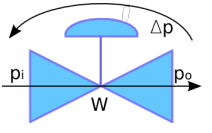
\includegraphics{img/valvola2.png}
\caption{Schema di una valvola}
\label{fig:valvola2}
\end{figure}
Le equazioni idrauliche e termiche sono rispettivamente:
$$
w=Cv_{max}\phi(x)\sqrt{\Delta p}
$$
$$T_i==T_o$$

\subsection{Scambi di calore}
\subsubsection{Scambio in un fluido}
\begin{figure}[tbh]
\centering
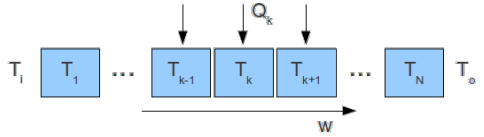
\includegraphics{img/flusso.png}
\caption{Scambio di calore in un fluido}
\label{fig:flusso}
\end{figure}
Per un fluido incomprimibile le equazioni di energia sono disaccoppiate da quelle idrauliche;dopo aver deciso la direzione del flusso le equazioni per ogni elemento sono descritte da:
$$\rho c V_k\dot{T_k}=wcT{k+1}-wcT_k+Q_k, \qquad T_{-1}=T_i, T_o=T_N$$
\subsubsection{Superfice metallica}
\begin{figure}[tbh]
\centering
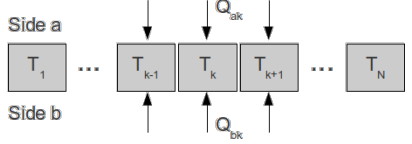
\includegraphics{img/metal2.png}
\caption{Scambio di calore con una superfice metallica}
\label{fig:metal2}
\end{figure}
Dividiamo il metallo nello stesso modo in cui abbiamo diviso il tubo in questo caso però l'equazione diventa:
$$\rho_mc_mV_{mk}\dot{T_k}=Q_{ak}+Q_{bk}$$
\subsubsection{Scambio convettivo}
\begin{figure}[tbh]
\centering
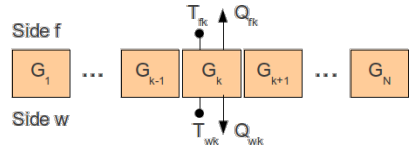
\includegraphics{img/convettivo2.png}
\caption{Scambio convettivo}
\label{fig:convettivo2}
\end{figure}
Per lo scambio convettivo adottiamo la stessa tecnica di discretizzazione perciò l'equazione di bilancio dell'energia diventa:
$$Q_{fk}=-Q_{wk}= \gamma S_k(T_{fk}-T_{wk})$$
dove il pedice "w" sta ad indicare il materiale di scambio e $S_k$ è la superfice di scambio.
